\documentclass[11pt]{article}
\usepackage{eacl2009}
\usepackage{times}
\usepackage[obeyspaces]{url}
\urlstyle{rm}
\usepackage{latexsym}
%\setlength\titlebox{6.5cm}    % You can expand the title box if you really have to
\usepackage{graphicx}
\usepackage{alltt}
\usepackage[T1]{fontenc}
\usepackage[utf8]{inputenc}
\usepackage{textcomp}  % to allow arrows
\usepackage{verbatim}
\usepackage[margin=10pt,font=small,labelfont=bf,labelsep=endash,center]{caption}

%\setlength{\intextsep}{1.5mm}  % tweaks the space between figures
%\setlength{\belowcaptionskip}{-2mm}

\interfootnotelinepenalty=10000

\title{Using constraint grammar in the Bangor Autoglosser\\ to disambiguate multilingual spoken text}

\author{Kevin Donnelly \textit{and} Margaret Deuchar\\
  ESRC Centre for Research on Bilingualism in Theory and Practice\\
  Prifysgol Bangor University, Wales, UK\\
  {\tt \{k.donnelly|m.deuchar\}@bangor.ac.uk}  }
\date{}

\begin{document}
\maketitle
\begin{abstract}
We present a novel use of constraint grammar (CG) in automatic glossing software to disambiguate surface forms in connected multilingual speech.  The resulting autoglosser output shows 97-99\% accuracy over all three languages.  We discuss the CG rules that help deliver this, noting the differences between those applying to Welsh and Spanish, and those applying to English.
\end{abstract}


\smallskip
\section{Introduction}
\label{sec:intro}


Bangor University's ESRC Centre for Research on Bilingualism,\footnote{http://bilingualism.bangor.ac.uk} established in Jnauary 2007, has assembled some 130 bilingual conversations in three corpora: \textbf{Siarad}\footnote{Siarad means ``speak'' in Welsh.} (Welsh-English), \textbf{Patagonia} (Welsh-Spanish), \textbf{Miami} (Spanish-English).

The conversations total some 80 hours and 750,000 words, and are all available under the GNU GPL.\footnote{http://www.gnu.org/licenses/gpl.html}  Each recording is provided with a detailed transcription in the widely-used CLAN format\footnote{http://childes.psy.cmu.edu/clan.  Note that using CLAN to record bilingual speech is an extension of its original focus on recording language development in children.} \cite{macwhinney2000}, along with a free translation in English, and an interlinear gloss giving lexemes and part-of-speech (POS) tags for each word, so that researchers without first-hand knowledge of the languages concerned can more easily parse the utterances.

\begin{table}[!hbtp]
\centering
\begin{tabular}{ccccc}
& \begin{small}\textit{Chats}\end{small} & \begin{small}\textit{Hours}\end{small} & \begin{small}\textit{Words}\end{small} & \begin{small}\textit{Date}\end{small} \\
\cline{1-5}\noalign{\smallskip}
\textbf{Welsh-English} & 69 & 40 & 456k & 2009 \\
\textbf{Welsh-Spanish} & 32 & 20 & 183k & 2011 \\
\textbf{Spanish-English} & 31 & 20 & 126k & 2011 \\
\hline\noalign{\smallskip}
& \textbf{132} & \textbf{80} & \textbf{765k} \\
\end{tabular}
\caption{The three ESRC Centre corpora.}
\label{corpora}
\end{table}

Part of a typical transcription is shown in Figure \ref{chat_file1}, in which (using CLAN terminology) three ``tiers'' can be discerned: the speech tier, the gloss tier, and the translation tier.

The speech tier (the words actually uttered) is marked by an initial ID to distinguish the speaker (e.g. \textit{*SER}), followed by the transcribed speech (with each word tagged for language\footnote{The autoglosser handles 4 marking systems, which reflect changes in transcription practice in the ESRC Centre over the past 5 years, and developments in CLAN itself.} -- unmarked for Welsh, \textit{@s:eng} for English, \textit{@s:cym\&eng} for indeterminate\footnote{Words which are used in both languages, and which therefore cannot be assigned unambiguously to one of them.}), and a tag (\textit{\%snd}) giving the time-location of the utterance in the audiofile.

The gloss tier is marked by an initial \textit{\%gls}, followed by a series of lexeme+POS-tag strings.

The translation tier is marked by an initial \textit{\%eng}, and gives a free translation of the speech tier (the speaker's utterance) into English.

\begin{figure*} 
\begin{footnotesize}
\begin{alltt}
\normalfont
*SER: dw i (y)n hopeless@s:eng efo tynnu llun . %snd:"deuchar1"_72848_73881
%gls: be.1S.PRES PRON.1S PRT hopeless with take.NONFIN picture
%eng: I'm hopeless at drawing
*SER: dw i (y)n tynnu llun i [/] i (y)r plant <i plant> [//] <i (y)r> [//] # i er@s:cym&eng &h Helen@s:cym&eng a Susanna@s:cym&eng a +/. %snd:"deuchar1"_73881_79477
%gls: be.1S.PRES PRON.1S PRT take.NONFIN picture for for DET children for children for DET for IM Helen and Susanna and
%eng: I draw a picture for ... for the children, for, er, Helen and Susanna and ...
\end{alltt}
\end{footnotesize}
\caption{Excerpt from the file \textit{deuchar1} in the Siarad corpus (Welsh-English).}
\label{chat_file1}
\end{figure*}

The corpora are valuable in examining how language is actually used: for instance, the differences between spoken language and formal written language, sociolinguistic variation (what forms of language are used where and by whom), the balance between languages in bilingual usage, and how one language handles lexical items from the other.\footnote{For instance,  \cite{stammers2010} has used the Siarad corpus to show that Welsh loan-verbs such as \textit{textio} (to text) behave more like ordinary Welsh verbs the more frequent they are.}

Manual glossing of the Siarad (Welsh-English) proved to be tedious and time-consuming, so in order to save valuable specialist time it was decided to explore automating the glossing of the Miami (Spanish-English) and Patagonia (Welsh-Spanish) corpora.

Although the CLAN project provides a tagging system (MOR),\footnote{http://childes.psy.cmu.edu/morgrams} this only caters for 11 languages, each with more than 5m speakers.  Vocabulary is distributed over a number of files, and MOR requires a separate pass over the file to tag each language.  Post-tagging disambiguation (using the POST program) is only available for 4 languages.  Software such as Toolbox\footnote{http://www.sil.org/computing/toolbox} offers interlinear glossing capability, but is aimed more at linguistic field researchers, and is less applicable to fully-described languages; moreover, it does not seem to be scriptable, which was essential in order to deal with the volume of data in the corpora.

There appears to be no tagger available at all for Welsh, reflecting the dearth of linguistic tools available to many minority languages \cite{antonsen2010}.

With no existing software meeting the purpose, a two-week test project in April 2010 looked at the viability of simply writing out entries from Spanish and Welsh dictionaries (see Section \ref{sec:dictionaries} below) for each word in the transcription.  The results of the tests were encouraging, and the only remaining issue was how to dismbiguate between the returned entries.  For this we turned to constraint grammar, and the remainder of this paper reports on how this is used in the autoglossing software developed over the past year.


\section{The dictionaries}
\label{sec:dictionaries}


A key element of any tagging or glossing system is the use of a dictionary to allow lookup of the word in the chosen language.
  
The Spanish dictionary used in the Autoglosser is based on the one used in Apertium,\footnote{http://apertium.org} a free (GPL) platform for developing rule-based machine translation systems.  The Welsh dictionary is based on Eurfa,\footnote{http://eurfa.org.uk} developed by the first author a few years ago, and still the largest free (GPL) dictionary for Welsh.  The English dictionary is based on Kevin Atkinson's Moby list.\footnote{http://wordlist.sourceforge.net}

The use of material with a free or public domain license allows existing lexical resources to be easily adapted and extended for the Autoglosser without having to worry about licensing terms.  This is an especially important consideration for minority languages like Welsh,\cite{streiter2006} where resources may be limited.

Each dictionary takes the form of one PostgreSQL database table, storing full words (not morphemes).  All of the original dictionaries have undergone some refactoring to simplify and standardise their layout, and to correct errors and omissions.\footnote{The English dictionary is particularly prone to include non-existent ``words'' such as \textit{fam}, \textit{fath}, \textit{gaster}, etc, and further cleaning is still required.}

The dictionary table can be easily edited in place, or it can be exported to a CSV file, making it accessible via a spreadsheet for those who are unfamiliar with databases.  The dictionary is therefore easy to update, since the format is a familiar glossary-style list of words.  This makes expanding or editing the dictionary more accessible for people without extensive computer skills, which is again important for minority languages -- no esoteric rules on word-division apply, nor are the contents distributed over several files.

In theory at least, this should simplify the addition of further languages in the future.  If a simple wordlist is available, it is possible to plug it into the autoglosser, and get some useful non-disambiguated output immediately; this output can then be progressively refined by the addition of CG rules,\footnote{Constraint grammar has been described as ``the only grammar-based parser framework'' (\url{http://giellatekno.uit.no/cg/11/index.html}), and it is indeed very easy for linguists to work with.} and refactoring of the dictionary lookup to allow a reduction in the size of the dictionaries. 

Some entries from the Welsh dictionary are in Table \ref{welsh_dict}.  The enlemma column gives the English lexeme for the word, and the pos column gives the part-of-speech (POS).

\begin{table}[!hbtp]
\centering
\begin{scriptsize}
\begin{tabular}{ccccccc}
\textit{surface} & \textit{lemma} & \textit{enlemma} & \textit{pos} & \textit{gender} & \textit{number} & \textit{tense} \\
\textbf{bara} & bara & bread & n & m & sg & \\
\textbf{cathod} & cath & cat & n & f & pl & \\
\textbf{mynd} & mynd & go & v & & & infin \\
\textbf{aeth} & mynd & go & v & & 3s & past \\
\textbf{hapus} & hapus & happy & adj & &  & \\
\textbf{rhywsut} & rhywsut & somehow & adv & & & \\
\textbf{heb} & heb & without & prep & & & \\
\end{tabular}
\end{scriptsize}
\caption{Entries from the Welsh dictionary.}
\label{welsh_dict}
\end{table}

A similar set of entries from the Spanish dictionary is in Table \ref{spanish_dict} -- it can be seen that the same columns are used in both dictionaries.

\begin{table}[!hbtp]
\centering
\begin{scriptsize}
\begin{tabular}{ccccccc}
\textit{surface} & \textit{lemma} & \textit{enlemma} & \textit{pos} & \textit{gender} & \textit{number} & \textit{tense} \\
\textbf{perro} & perro & dog & n & m & sg & \\
\textbf{canciones} & canción & song & n & f & pl & \\
\textbf{empezar} & empezar & start & v & & & infin \\
\textbf{empieza} & empezar & start & v & & 23s & pres \\
\textbf{empieza} & empezar & start & v & & 2s & imper \\
\textbf{rojo} & rojo & red & adj & m & sg & \\
\textbf{rojas} & rojo & red & adj & f & pl & \\
\textbf{por} & por & for & prep & & & \\
\end{tabular}
\end{scriptsize}
\caption{Entries from the Spanish dictionary.}
\label{spanish_dict}
\end{table}

Both Spanish and Welsh are inflected languages, where the surface forms give clues about the word's POS.  English, however, is an analytic language where the POS of the many homophonous words is defined by their role in the sentence.  The format for the English dictionary, some entries for which are in Table \ref{english_dict}, reflects this by having the POS reflect all of these possibilities, with the correct POS being selected during disambiguation.  For example, \textbf{walk} can be a noun (\textit{a short walk}), an imperative verb (\textit{walk the line!}), an infinitive verb (\textit{to walk a mile}) and a present tense verb (\textit{they walk everywhere}).  Thus \textbf{walk} has the POS \textbf{sv}, meaning that it can be either a singular noun or a verb. The main benefit of this approach is that it minimises the number of entries which the dictionary has to include (in this case, one entry instead of four), and therefore makes maintenance of the dictionary easier.

\begin{table}[!hbtp]
\centering
\begin{scriptsize}
\begin{tabular}{ccccccc}
\textit{surface} & \textit{lemma} & \textit{pos} & \textit{number} & \textit{tense} \\
\textbf{walk} & walk & sv & & infin \\
\textbf{break} & break & sv & & infin \\
\textbf{broke} & break & av & & past \\
\textbf{broken} & break & av & & pastpart \\
\textbf{car} & car & n & sg & \\
\textbf{quick} & adj & & & \\
\textbf{by} & by & prep & & \\
\textbf{which} & which & rel & & \\
\end{tabular}
\end{scriptsize}
\caption{Entries from the English dictionary.}
\label{english_dict}
\end{table}


\section{The autoglossing process}
\label{sec:autoglosser}


Each line of the transcribed conversation file is read into an utterances table containing the following fields:
\vspace{-3mm}
\begin{itemize}
\setlength{\itemsep}{-2mm}
\item utterance\_id
\item filename
\item speaker
\item surface (the utterance)
\item startpoint
\item endpoint
\item duration
\item manual gloss (if present)
\item English translation (if present)
\item comments (if present)
\item precode\footnote{This marks entire utterances in the least-frequent language of the conversation.} (if present)
\end{itemize}

Any non-lexical markers in the utterance are discarded, and it is then split into words, which are stored in a words table with the following fields:
\vspace{-3mm}
\begin{itemize}
\setlength{\itemsep}{-2mm}
\item word\_id
\item utterance\_id
\item location of the word in the utterance
\item surface (the word)
\item automatic gloss (to hold the later output)
\item manual gloss (if present)
\item language id
\item speaker
\item filename
\end{itemize}

Each entry in the words table is looked up against the dictionary table for the appropriate language, using the language assigned to the word by the transcriber.\footnote{In the absence of this, it would in principle be possible to use a brute-force lookup on each dictionary in turn.}

The lookup includes some basic segmentation of the word.  This helps to minimise the number of dictionary entries and make maintenance of the dictionary easier.

For Welsh, the lookup detects mutation\footnote{Mutation -- morphophonemic alteration of initial consonants, which also marks syntactic relations at the clause level -- is an important characteristic of the Celtic languages. A Welsh example is: \textbf{mae o'n marw} (\textit{he is dying}), but \textbf{mae o'n farw} (\textit{he is dead}), where the change \textbf{m$\rightarrow$f} signifies that the mutated word is an adjective and not a verb. These mutations have to be removed in order to get to the underlying lexeme.} and adds corresponding tags:

\noindent
\hangindent=2em
\hangafter=0
\textbf{thad} \textrightarrow \textbf{tad} (\textit{father}) + am (aspirate mutation) \\
\textbf{gael} \textrightarrow \textbf{cael} (\textit{get}) + sm (soft mutation) 

For Spanish, tags are added when clitic pronouns attached to verbforms are detected:

\noindent
\hangindent=2em
\hangafter=0
\textbf{ponerle} \textrightarrow \textbf{poner} (\textit{put}) + \textbf{le}[pron.mf.3s] \\
\textbf{déjanos} \textrightarrow \textbf{déja} (\textit{leave}) + \textbf{nos}[pron.mf.1p]
                                                                  
For English, tags are added for things like:

\noindent
(a) elisions:

\noindent
\hangindent=2em
\hangafter=0
\textbf{gonna} \textrightarrow \textbf{go} \# to.prep \\
\textbf{we're} \textrightarrow \textbf{we} \# be.v.pres

\noindent
(b) genitives or verb elisions:

\noindent
\hangindent=2em
\hangafter=0
\textbf{father's} \textrightarrow \textbf{father} \# gb

\noindent
(c) plural nouns or 3s present tense verbs:

\noindent
\hangindent=2em
\hangafter=0
\textbf{breaks} \textrightarrow \textbf{break} \# pv

\noindent
(d) adjectives or past tense verbs:

\noindent
\hangindent=2em
\hangafter=0
\textbf{constructed} \textrightarrow \textbf{construct} \# av

\noindent
(e) adjectives, singular nouns or present participle verbs:

\noindent
\hangindent=2em
\hangafter=0
\textbf{thinking} \textrightarrow \textbf{think} \# asv

\noindent
(f) adverbs:

\noindent
\hangindent=2em
\hangafter=0
\textbf{quickly} \textrightarrow \textbf{quick} \# adv

All matching entries in the dictionary are then written out to a file in the format required by the contraint grammar parser.\footnote{http://visl.sdu.dk/cg3.html}  Figures \ref{welsh_before} and \ref{english_before} show the output after lookup of a monolingual phrase in Welsh and English respectively.

\vspace{-2mm}
\begin{figure}[!hbtp]
\centering
\begin{footnotesize}
\begin{alltt}
\normalfont
"<ddim>"
    "dim"  {96,1} [cy] n m sg :nothing: + sm
    "dim"  {96,1} [cy] adv :not: + sm
"<yn>"
    "yn"  {96,2} [cy] stat :stative: 
    "yn"  {96,2} [cy] prep :in: 
    "gan"  {96,2} [cy] prep :with: + sm
"<gynnar>"
    "cynnar"  {96,3} [cy] adj :early: + sm
"<iawn>"
    "iawn"  {96,4} [cy] adv :OK:
    "iawn"  {96,4} [cy] adv :very:
\end{alltt}
\end{footnotesize}
\caption{A phrase, after lookup and before disambiguation, meaning ``\textit{not very early}'', from the file \textit{patagonia1} in the Patagonia corpus (Welsh-Spanish).}
\label{welsh_before}
\end{figure}

\vspace{-5mm}
\begin{figure}[!hbtp]
\centering
\begin{footnotesize}
\begin{alltt}
\normalfont
"<it's>"
    "it"  {545,1} [en] pron.sub 3s :it: # gb
"<coming>"
    "come"  {545,2} [en] sv infin :come: # asv
"<out>"
    "out"  {545,3} [en] adv :out:
"<on>"
    "on"  {545,4} [en] prep :on:
"<D_V_D>"
    "D_V_D"  {545,5} [en] name
"<then>"
    "then"  {545,6} [en] adv :then:
\end{alltt}
\end{footnotesize}
\caption{A phrase, after lookup and before disambiguation, from the file \textit{herring7} in the Miami corpus (Spanish-English).}
\label{english_before}
\end{figure}

The constraint grammar parser applies the rules in the grammar file to discard invalid entries and convert tags where appropriate, and creates another file containing only valid, disambiguated entries.  The two phrases given above are shown after disambiguation in Figures \ref{welsh_after} and \ref{english_after}.

\vspace{-2mm}
\begin{figure}[!hbtp]
\centering
\begin{footnotesize}
\begin{alltt}
\normalfont
"<ddim>"
    "dim" {96,1} [cy] adv :not: + sm
"<yn>"
    "yn" {96,2} [cy] stat :stative:
"<gynnar>"
    "cynnar" {96,3} [cy] adj :early: + sm
"<iawn>"
    "iawn" {96,4} [cy] adv :very:
\end{alltt}
\end{footnotesize}
\caption{The Welsh phrase from Figure \ref{welsh_before} after disambiguation.}
\label{welsh_after}
\end{figure}

\vspace{-5mm}
\begin{figure}[!hbtp]
\centering
\begin{footnotesize}
\begin{alltt}
\normalfont
\textbf{"<it's>"}
    "it" {545,1} [en] pron.sub 3s :it: # be.v.3s.pres
\textbf{"<coming>"}
    "come" {545,2} [en] v prespart :come: #
\textbf{"<out>"}
    "out" {545,3} [en] adv :out:
\textbf{"<on>"}
    "on" {545,4} [en] prep :on:
\textbf{"<D_V_D>"}
    "D_V_D" {545,5} [en] name
\textbf{"<then>"}
    "then" {545,6} [en] adv :then:
\end{alltt}
\end{footnotesize}
\caption{The English phrase from Figure \ref{english_before} after disambiguation.}
\label{english_after}
\end{figure}

This file is then read into the database, and the glosses (in the form of a lexeme+POS-tag string, following the Leipzig schema \cite{leipzig2008} so far as possible) are extracted and stored in the words table against each word of the original transcription.  At this point, the words table looks like Figure \ref{words_db}, where the words in a Spanish utterance meaning ``\textit{And if some lorry goes in there, for example, to leave off furniture or whatever.}'' have all been glossed appropriately.

\begin{figure}[!hbtp]
\centering
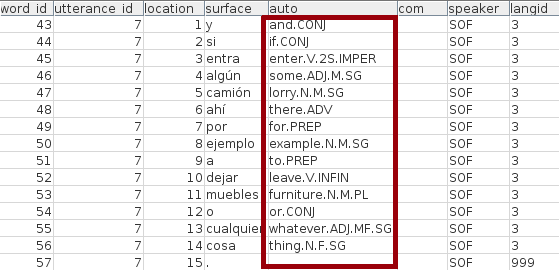
\includegraphics[scale=0.5]{words_table.png}
\caption{An utterance from the words table for the file \textit{sastre1} in the Miami corpus (Spanish-English)}
\label{words_db}
\end{figure}

Finally, a text with an interlinear gloss, as in Figure \ref{chat_file2}, is created by writing out the utterances again, along with the concatenated glosses.  Comparing to Figure \ref{chat_file1}, an additional \textit{\%aut} tier has been added for each utterance, in parallel with the pre-existing \textit{\%gls} tier provided by manual glossing.

\begin{figure*}[!hbtp]
\begin{footnotesize}
\begin{alltt}
\normalfont
*SER:   dw i (y)n hopeless@s:eng efo tynnu llun . %snd:"deuchar1"_72848_73881
%aut:   be.V.1S.PRES.SPOKEN I.PRON.1S stative.STAT hopeless.ADJ with.PREP take.V.INFIN picture.N.M.SG 
%gls:   be.1S.PRES PRON.1S PRT hopeless with take.NONFIN picture
%eng:   I'm hopeless at drawing
*SER:   dw i (y)n tynnu llun i [/] i (y)r plant <i plant> [//] <i (y)r> [//] # i er@s:cym&eng &h Helen@s:cym&eng a Susanna@s:cym&eng a +/ . %snd:"deuchar1"_73881_79477
%aut:   be.V.1S.PRES.SPOKEN I.PRON.1S stative.STAT take.V.INFIN picture.N.M.SG to.PREP to.PREP the.DET.DEF children.N.M.PL to.PREP children.N.M.PL to.PREP the.DET.DEF to.PREP er.IM name and.CONJ name and.CONJ 
%gls:   be.1S.PRES PRON.1S PRT take.NONFIN picture for for DET children for children for DET for IM Helen and Susanna and
%eng:   I draw a picture for...for the children, for, er Helen and Susanna and...
\end{alltt}
\end{footnotesize}
\caption{Autoglossed excerpt from the file \textit{deuchar1} in the Siarad corpus (Welsh-English) -- compare Figure \ref{chat_file1}.}
\label{chat_file2}
\end{figure*}

The Autoglosser produces glossed text at a rate of 900-1100 words per minute (depending on whether the original transcription file already contains a manual gloss tier).  The transcription of a half-hour conversation can therefore be glossed in around 6 minutes.\footnote{The entire Siarad corpus of around 40 hours duration (456,000 words) was glossed in 8h27m.} 

The grammar file currently contains about 500 rules for Welsh, about 200 for English, and around 170 for Spanish.  These figures reflect the fact that most work so far has been done on Welsh.

Preliminary results (see Table \ref{accuracy}) suggest that the Autoglosser's accuracy is 97-99\%, depending on the language.  We are confident that the accuracy rate can be further improved.

\begin{table*}[!hbtp]
\centering
\begin{tabular}{ccccccc}
& \begin{small}\textit{Corpus}\end{small} & \begin{small}\textit{Files}\end{small} & \begin{small}\textit{Words}\end{small} & \begin{small}\textit{Accuracy}\end{small} & \begin{small}\textit{MCL}\end{small} & \begin{small}\textit{Coverage}\end{small} \\
\cline{2-7}\noalign{\smallskip}
\textbf{Welsh-Spanish} & Patagonia & patagonia1, 2, 3, 6 & 15,677 & 99\% & W (92\%) & 100\% \\
\textbf{Welsh-English} & Siarad & stammers4, deuchar1 & 10,411 & 98\% & W (81\%) & 96\% \\
\textbf{Spanish-English} & Miami & zeledon5 & 4,202 & 97\% & S (59\%) & 97\% \\
\end{tabular}
\caption[center]{Autoglossing accuracy and coverage for sample files from the three ESRC Centre corpora.  In the MCL (most common language) column, W=Welsh and S=Spanish.  Coverage is 100\% for the Patagonia files because all unknown words were added to the dictionaries before autoglossing.}
\label{accuracy}
\end{table*}


\section{Using constraint grammar}
\label{sec:constraint}


We discuss here two issues:
\begin{itemize}
\item The addition of tags in the lookup output to specify language, and the handling of these in the grammar so as to allow one-pass disambiguation of multilingual text.
\item The different approaches taken in the grammar to handle the differing nature of the languages (already reflected to some extent in the dictionary entries).
\end{itemize}


\subsection{Language-specific rules}
\label{sec:langspec}


Multilingual discourse is far more common than has been assumed in classical linguistics, and it is only over the last 20 years that this important area has been given proper attention.  The Autoglosser is the first attempt to apply constraint grammar to multilingual text, and in fact only two things need to be done: (1) include the language tag in the output from each word's lookup; (2) put all the rules (grouped according to language for ease of reference) into the same grammar file. 

In Figure \ref{bilingual}, the phrase oscillates between Welsh and Spanish, and this is reflected in the inclusion of the tags \textbf{[cy]} and \textbf{[es]} in the readings.

\begin{figure}[!hbtp]
\centering
\begin{footnotesize}
\begin{alltt}
\normalfont
\textbf{"<mewn>"}
    "mewn" {128,4} [cy] prep :in:
\textbf{"<motor>"}
    "motor" {128,5} [es] n m sg :motor:
\textbf{"<newydd>"}
    "newydd" {128,6} [cy] adj :new:
\textbf{"<internacional>"}
    "internacional" {128,7} [es] adj mf sg :internat\-ional:
\end{alltt}
\end{footnotesize}
\caption{A bilingual phrase (\textit{``in a new international car''}) from the file \textit{patagonia2} in the Patagonia corpus (Welsh-Spanish).}
\label{bilingual}
\end{figure}

In the following noun phrases, the last word (\textbf{dro}, \textbf{man}, \textbf{viaje}) can be both a noun and a verb.
\indent Welsh: \textbf{yr ail dro} (\textit{the second time}) \\
\indent English: \textbf{the third man} \\
\indent Spanish: \textbf{el primer viaje} (\textit{the first journey}) \\
A rule such as: \\
\indent\textbf{select (n) if (-1 (ord));} \\
will choose the noun (\textbf{n}) reading if the first word to the left (\textbf{-1}) is an ordinal (\textbf{ord}), meaning that the verb readings for \textbf{dro}, \textbf{man} and \textbf{viaje} will be deleted.

The language tag can be used to constrain the application of the constraint grammar rules to the relevant language.\footnote{In practice, there is only a small number of cases where full constraint of the rules is essential (because only a couple of dozen words in each language overlap orthographically), but it is prudent at this stage to err on the side of over-specification.}  Thus, if the above rule is amended to read:\\
\indent\textbf{select ([es] n) if (-1 ([es] ord));} \\
it will only apply to the Spanish phrase, and not to the Welsh or English ones, meaning that the verb reading will still be available in those languages.

It is also possible to make the rules apply across language boundaries by selectively removing language constraints.

In Figure \ref{otro}, the Spanish \textbf{otro} can be either an adjective before a noun, or a pronoun.  If the selection rule leaves the noun unspecified as to language: \\
\indent\textbf{select ([es] adj) if (-1 (ord));} \\
the adjective reading will be selected before any noun (not just Spanish nouns), as in Figure \ref{otro1}.

\begin{figure}[!hbtp]
\centering
\begin{footnotesize}
\begin{alltt}
\normalfont
\textbf{"<es>"}
    "ser"  {500,1} [es] v 23s pres :be:
\textbf{"<otro>"}
    "otro"  {500,2} [es] adj m sg :other:
    "otro"  {500,2} [es] pron m sg :other:
\textbf{"<zip>"}
    "zip"  {500,3} [en] n sg :zip:
\textbf{"<code>"}
    "code"  {500,4} [en] n sg :code:
\end{alltt}
\end{footnotesize}
\caption{A bilingual phrase (\textit{``it's a different zipcode''}) from the file \textit{sastre1} in the Miami corpus (Spanish-English).}
\label{otro}
\end{figure}

\begin{figure}[!hbtp]
\centering
\begin{footnotesize}
\begin{alltt}
\normalfont
\textbf{"<es>"}
    "ser"  {500,1} [es] v 23s pres :be:
\textbf{"<otro>"}
    "otro"  {500,2} [es] adj m sg :other:
\textbf{"<zip>"}
    "zip"  {500,3} [en] n sg :zip:
\textbf{"<code>"}
    "code"  {500,4} [en] n sg :code:
\end{alltt}
\end{footnotesize}
\caption{The bilingual phrase from Figure \ref{otro} after disambiguation.}
\label{otro1}
\end{figure}

In Figure \ref{camping}, \textbf{camping} can be an adjective (\textit{the camping ground}), a singular noun (\textit{camping is fun}), or (as here) a verb.  In \textbf{vamos camping}, the \textbf{asv} tag can be converted to the desired present participle verb tag by referring to the meaning of the preceding verb, so that the rule applies to both English (\textit{go camping}) and Spanish (\textit{vamos camping}):

\noindent
\hangindent=1em
\hangafter=0
\textbf{substitute (sv infin asv) (v prespart) ([en] sv infin asv) (-1 (:go:));}

\noindent as in Figure \ref{camping1}.

\begin{figure}[!hbtp]
\centering
\begin{footnotesize}
\begin{alltt}
\normalfont
\textbf{"<cada>"}
    "cada"  {79,5} [es] adj mf sg :every:
\textbf{"<vez>"}
    "vez"  {79,6} [es] n f sg :time:
\textbf{"<que>"}
    "que"  {79,7} [es] conj :than:
    "que"  {79,7} [es] conj :that:
\textbf{"<nos>"}
    "yo"  {79,8} [es] pron.obl mf 1p :us:
\textbf{"<vamos>"}
    "ir"  {79,9} [es] v 1p pres :go:
\textbf{"<camping>"}
    "camp"  {79,10} [en] sv infin :camp: # asv
\end{alltt}
\end{footnotesize}
\caption{A bilingual phrase (\textit{``every time that we go camping''}) from the file \textit{sastre1} in the Miami corpus (Spanish-English).}
\label{camping}
\end{figure}


\subsection{Tidying readings}
\label{sec:tidying}


The re-use of lexical resources can lead to a conflict -- for many purposes, a comprehensive dictionary giving as many entries as possible for a particular word is desirable, but these multiple entries are not required for an application like the autoglosser, where one lemma will usually be sufficient for tagging purposes.

\begin{figure}[!hbtp]
\centering
\begin{footnotesize}
\begin{alltt}
\normalfont
\textbf{"<cada>"}
    "cada" {79,5} [es] adj mf sg :every:
\textbf{"<vez>"}
    "vez" {79,6} [es] n f sg :time:
\textbf{"<que>"}
    "que" {79,7} [es] pron.rel :that:
\textbf{"<nos>"}
    "yo" {79,8} [es] pron.obl mf 1p :us:
\textbf{"<vamos>"}
    "ir" {79,9} [es] v 1p pres :go:
\textbf{"<camping>"}
    "camp" {79,10} [en] v prespart :camp: #
\end{alltt}
\end{footnotesize}
\caption{The bilingual phrase from Figure \ref{camping} after disambiguation.}
\label{camping1}
\end{figure}

In cases where the entries are archaic or infrequent words, we use CG \textbf{select} rules to remove them from consideration.  The Welsh words \textbf{huno} (\textit{sleep}) and \textbf{pallu} (\textit{refuse}) are low-frequency, so the following rules are applied:

\noindent
\hangindent=1em
\hangafter=0
\textbf{remove ("huno" [cy] :sleep:);} \\
\textbf{remove ("pallu" v :refuse:);}

In other cases, where a single word has different meanings we use CG \textbf{select} rules to prioritise one of the meanings.  The Welsh dictionary gives two meanings for \textbf{cyfeiriad} (\textit{direction} and \textit{address}) -- the following rule ensures that the \textit{address} meaning is ignored:

\noindent
\hangindent=1em
\hangafter=0
\textbf{select ("cyfeiriad" [cy] :direction:);}

The lookup process can generate readings which are invalid, and these need to be removed.  The cohort of readings for the Welsh word \textbf{nos} (\textit{night}) will include an incorrect one interpreting it as a nasally-mutated form of the imperative (\textbf{dos)} of the verb \textbf{mynd} (\textit{go}), which is linguistically impossible.  This sort of entry can be removed with a rule like:

\noindent
\hangindent=1em
\hangafter=0
\textbf{remove ([cy] "mynd" v 2s imper nm);}

A similar issue arises when indeterminate words are being looked up.  It will be recalled that indeterminate words are those which appear in dictionaries of both languages, so it is impossible to state unequivocally which language they belong to.\footnote{This is meant diachronically rather than synchronically, in terms of current usage in both languages -- historically, the word may be considered a loanword.}  Since the practice in the transcriptions is to use English spelling for indeterminate words, lookup for these words uses the English dictionary.  The interaction with Welsh mutation can lead to invalid readings, such as the interpretation of the hesitation marker \textbf{um} as a soft-mutated form of the word gum, which is extremely unlikely.  This can be removed with a rule like:

\noindent
\hangindent=1em
\hangafter=0
\textbf{remove ([in] "gum" n sg sm);}


\subsection{Nature of rules}
\label{sec:nature}


Spanish and Welsh are inflected languages,\footnote{Though it should be noted that in Welsh, particularly spoken Welsh, inflected verbforms are now widely replaced by periphrastic forms.} while English is an analytic language with few inflections (mainly in ``strong'' verbs).  This is reflected in the nature of the rules that have proved most efficient in the autoglosser.

For Spanish and Welsh, surface forms are fairly well-defined by their shape -- \textbf{empieza}, for instance, can only be the second/third person singular present or the second person singular imperative of \textbf{empezar} (\textit{to begin}).  The lookup fetches these entries from the dictionary,\footnote{The possibility of de-conjugating inflected verbs on-the-fly is attractive, but may be too complex to attempt at this stage.} and so the rules consist mainly of \textbf{select} rules (with a few \textbf{remove}s and \textbf{substitute}s).

For English, on the other hand, the surface form gives us few clues about the part-of-speech a word belongs to, which is largely defined by its role in the sentence -- \textbf{break} can be a singular noun, or a verb infinitive, or the non-third person singular present tense.  Instead of giving \textbf{break} three entries in the English dictionary, we have chosen, as noted in Section  \ref{sec:dictionaries},  to assign it one entry, with a tag (\textit{sv}) which reflects this diversity of role.  

The result is that the the vast majority of rules for English are \textbf{substitute}s, converting one set of tags into another.  For example, the surface word \textbf{miniature} can be either an adjective or a singular noun, so it is tagged \textit{as} in the dictionary.  Rules such as the following then handle its correct tagging based on context:

\noindent
\hangindent=1em
\hangafter=0
\textbf{substitute (as) (adj) ([en] as) (1 ([en] n) or ([en] pron));}

\noindent This says that an English \textit{as} tag should be converted to an \textit{adjective} tag when the word is followed by a noun or pronoun (e.g. \textbf{a miniature rabbit}, \textbf{miniature ones}).


\subsection{Rule scope}
\label{sec:scope}


Rule types to avoid - 

Our current view is that \textbf{remove} and \textbf{select-if-not} rules are particularly problematic unless they are carefully constrained.  A select rule is exclusive in what it applies to, and it may be considered that it is possible to frame a select-if-not rule to be equally exclusive.  By its nature, however


\section{Further work}
\label{sec:further}


Although the current configuration of rules is working well, we hope to explore further refinement of the grammar.  This would include not only conflating similar rules within a language, but also seeking to use the grammar to mark clause relationships.  The latter would be of value in the further linguistic analysis of the influence of clause structure on language switching in bilingual discourse.


\section*{Acknowledgments}

The support of the Arts and Humanities Research Council (AHRC), the Economic and Social Research Council (ESRC), the Higher Education Funding Council for Wales and the Welsh Assembly Government is gratefully acknowledged. The work presented in this paper was part of the programme of the ESRC Centre for Research on Bilingualism in Theory and Practice at Bangor University.


\bibliography{autoglosser}
\bibliographystyle{acl}

\end{document}
